\documentclass{article}
\usepackage{amsmath}
\usepackage{tikz}
\usepackage{graphicx}

\begin{document}
\section*{8.26}
\subsection*{b)}
\paragraph{Specification:}
Check if these points form a right angled triangle:
\begin{align*}
    A(-1|-2) &&
    B(1|-3) &&
    C(4|2) \\[20pt]
\end{align*}

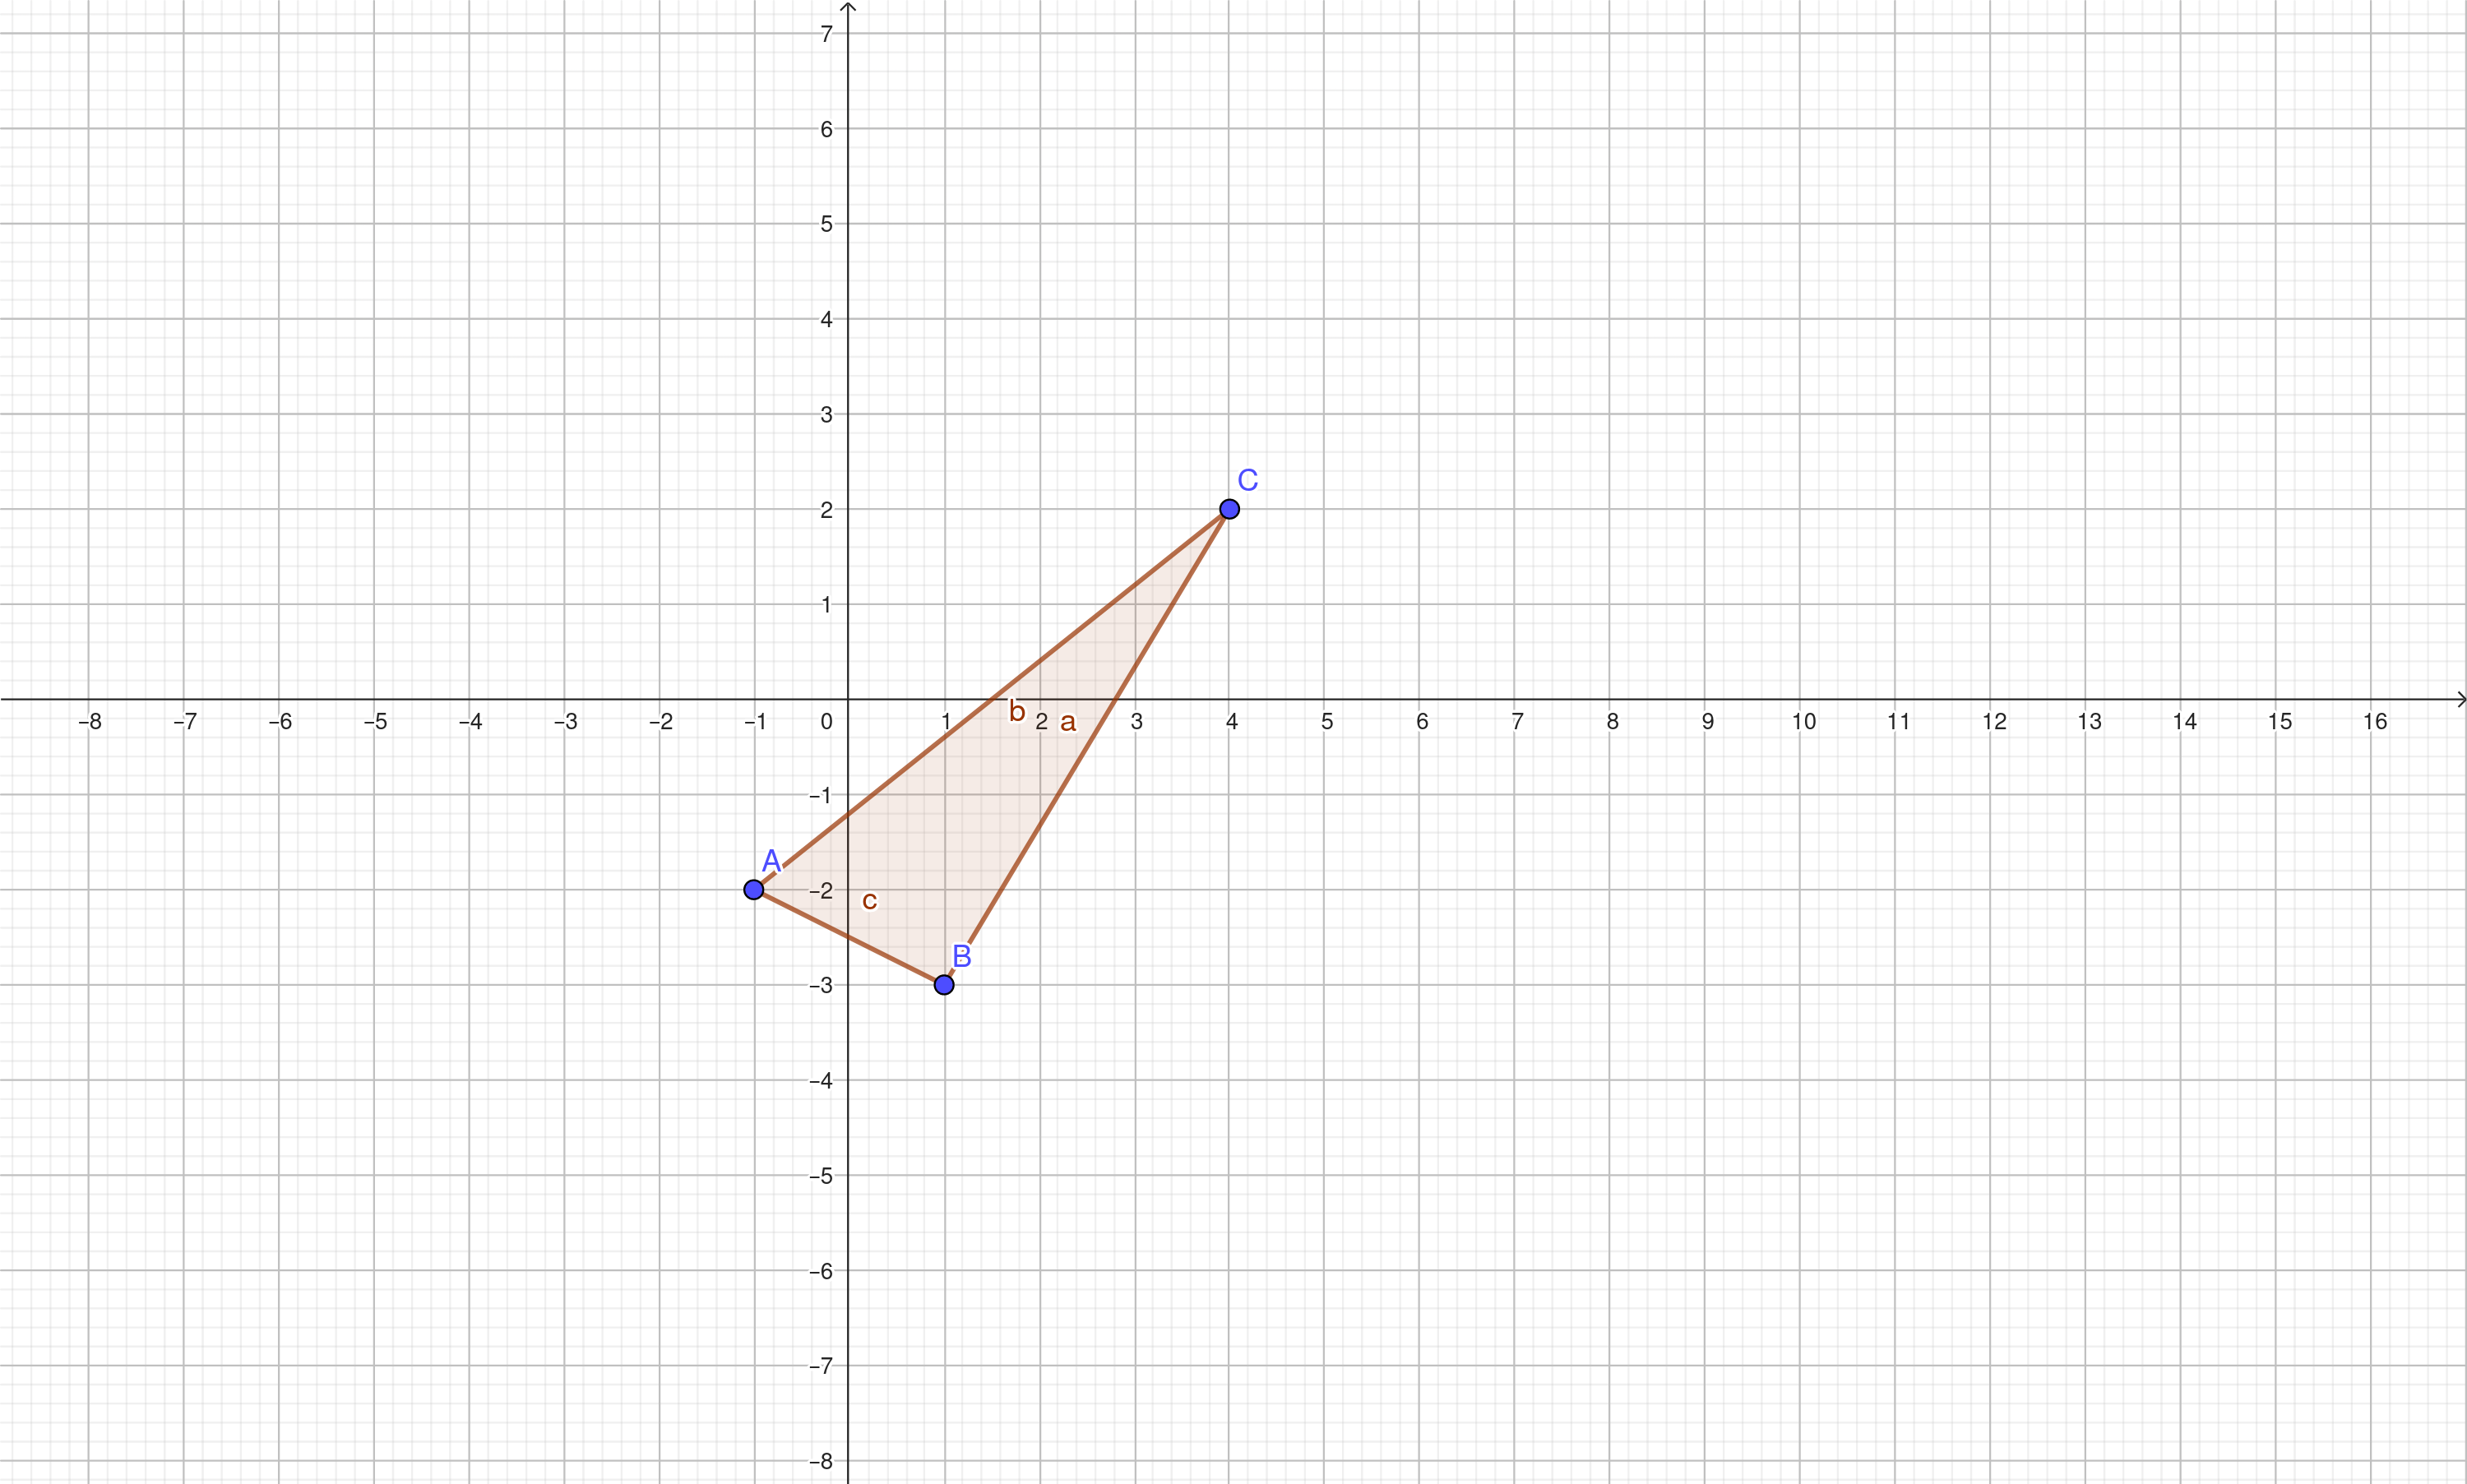
\includegraphics[width=\linewidth]{images/8-26-b.png}

\paragraph{Definitions:}
\begin{align*}
    \vec{a} &= \vec{BC} \\
    \vec{b} &= \vec{CA} \\
    \vec{c} &= \vec{AB} \\
\end{align*}

\paragraph{Exercises:}
\begin{align}
    \vec{a} \cdot \vec{b} &= a_x * b_x + a_y * b_y \\
    \vec{a} \cdot \vec{b} &= -1 * 1 + -2 * -3 \\
    \vec{a} \cdot \vec{b} &= -1 + 6 \\
    \vec{a} \cdot \vec{b} &= 5 \\[20pt]
    \vec{a} \cdot \vec{c} &= a_x * c_x + a_y * c_y \\
    \vec{a} \cdot \vec{c} &= -1 * 4 + -2 * 2 \\
    \vec{a} \cdot \vec{c} &= -4 + -4 \\
    \vec{a} \cdot \vec{c} &= -8 \\[20pt]
    \vec{a} \cdot \vec{c} &= b_x * c_x + b_y * c_y \\
    \vec{a} \cdot \vec{c} &= 1 * 4 + -3 * 2 \\
    \vec{a} \cdot \vec{c} &= 4 + -6 \\
    \vec{a} \cdot \vec{c} &= -2
\end{align}

\paragraph{Answer:}
The triangle is not a right angle as none of the angles $\alpha$, $\beta$, $\gamma$ are $90^\circ$.
This is shown be the fact that none of the dot products of the triangles sides are 0.

\pagebreak

\section*{8.29}
\subsection*{1)}
\paragraph{Specification:}
Find the mistake in the following equations:
 \def\AB{\begin{pmatrix}
       15 \\
       8 \\
    \end{pmatrix}}

\def\BC{\begin{pmatrix}
       -12 \\
       5 \\
    \end{pmatrix}}

\def\cosval{-0.633...}
\def\cosang{129.31}
\def\cosanginv{\pgfmathparse{180 - \cosang}\pgfmathresult}
\def\sinofang{\pgfmathparse{sin(\cosang)}\pgfmathresult}
\def\sinofanginv{\pgfmathparse{sin(180 - \cosang)}\pgfmathresult}

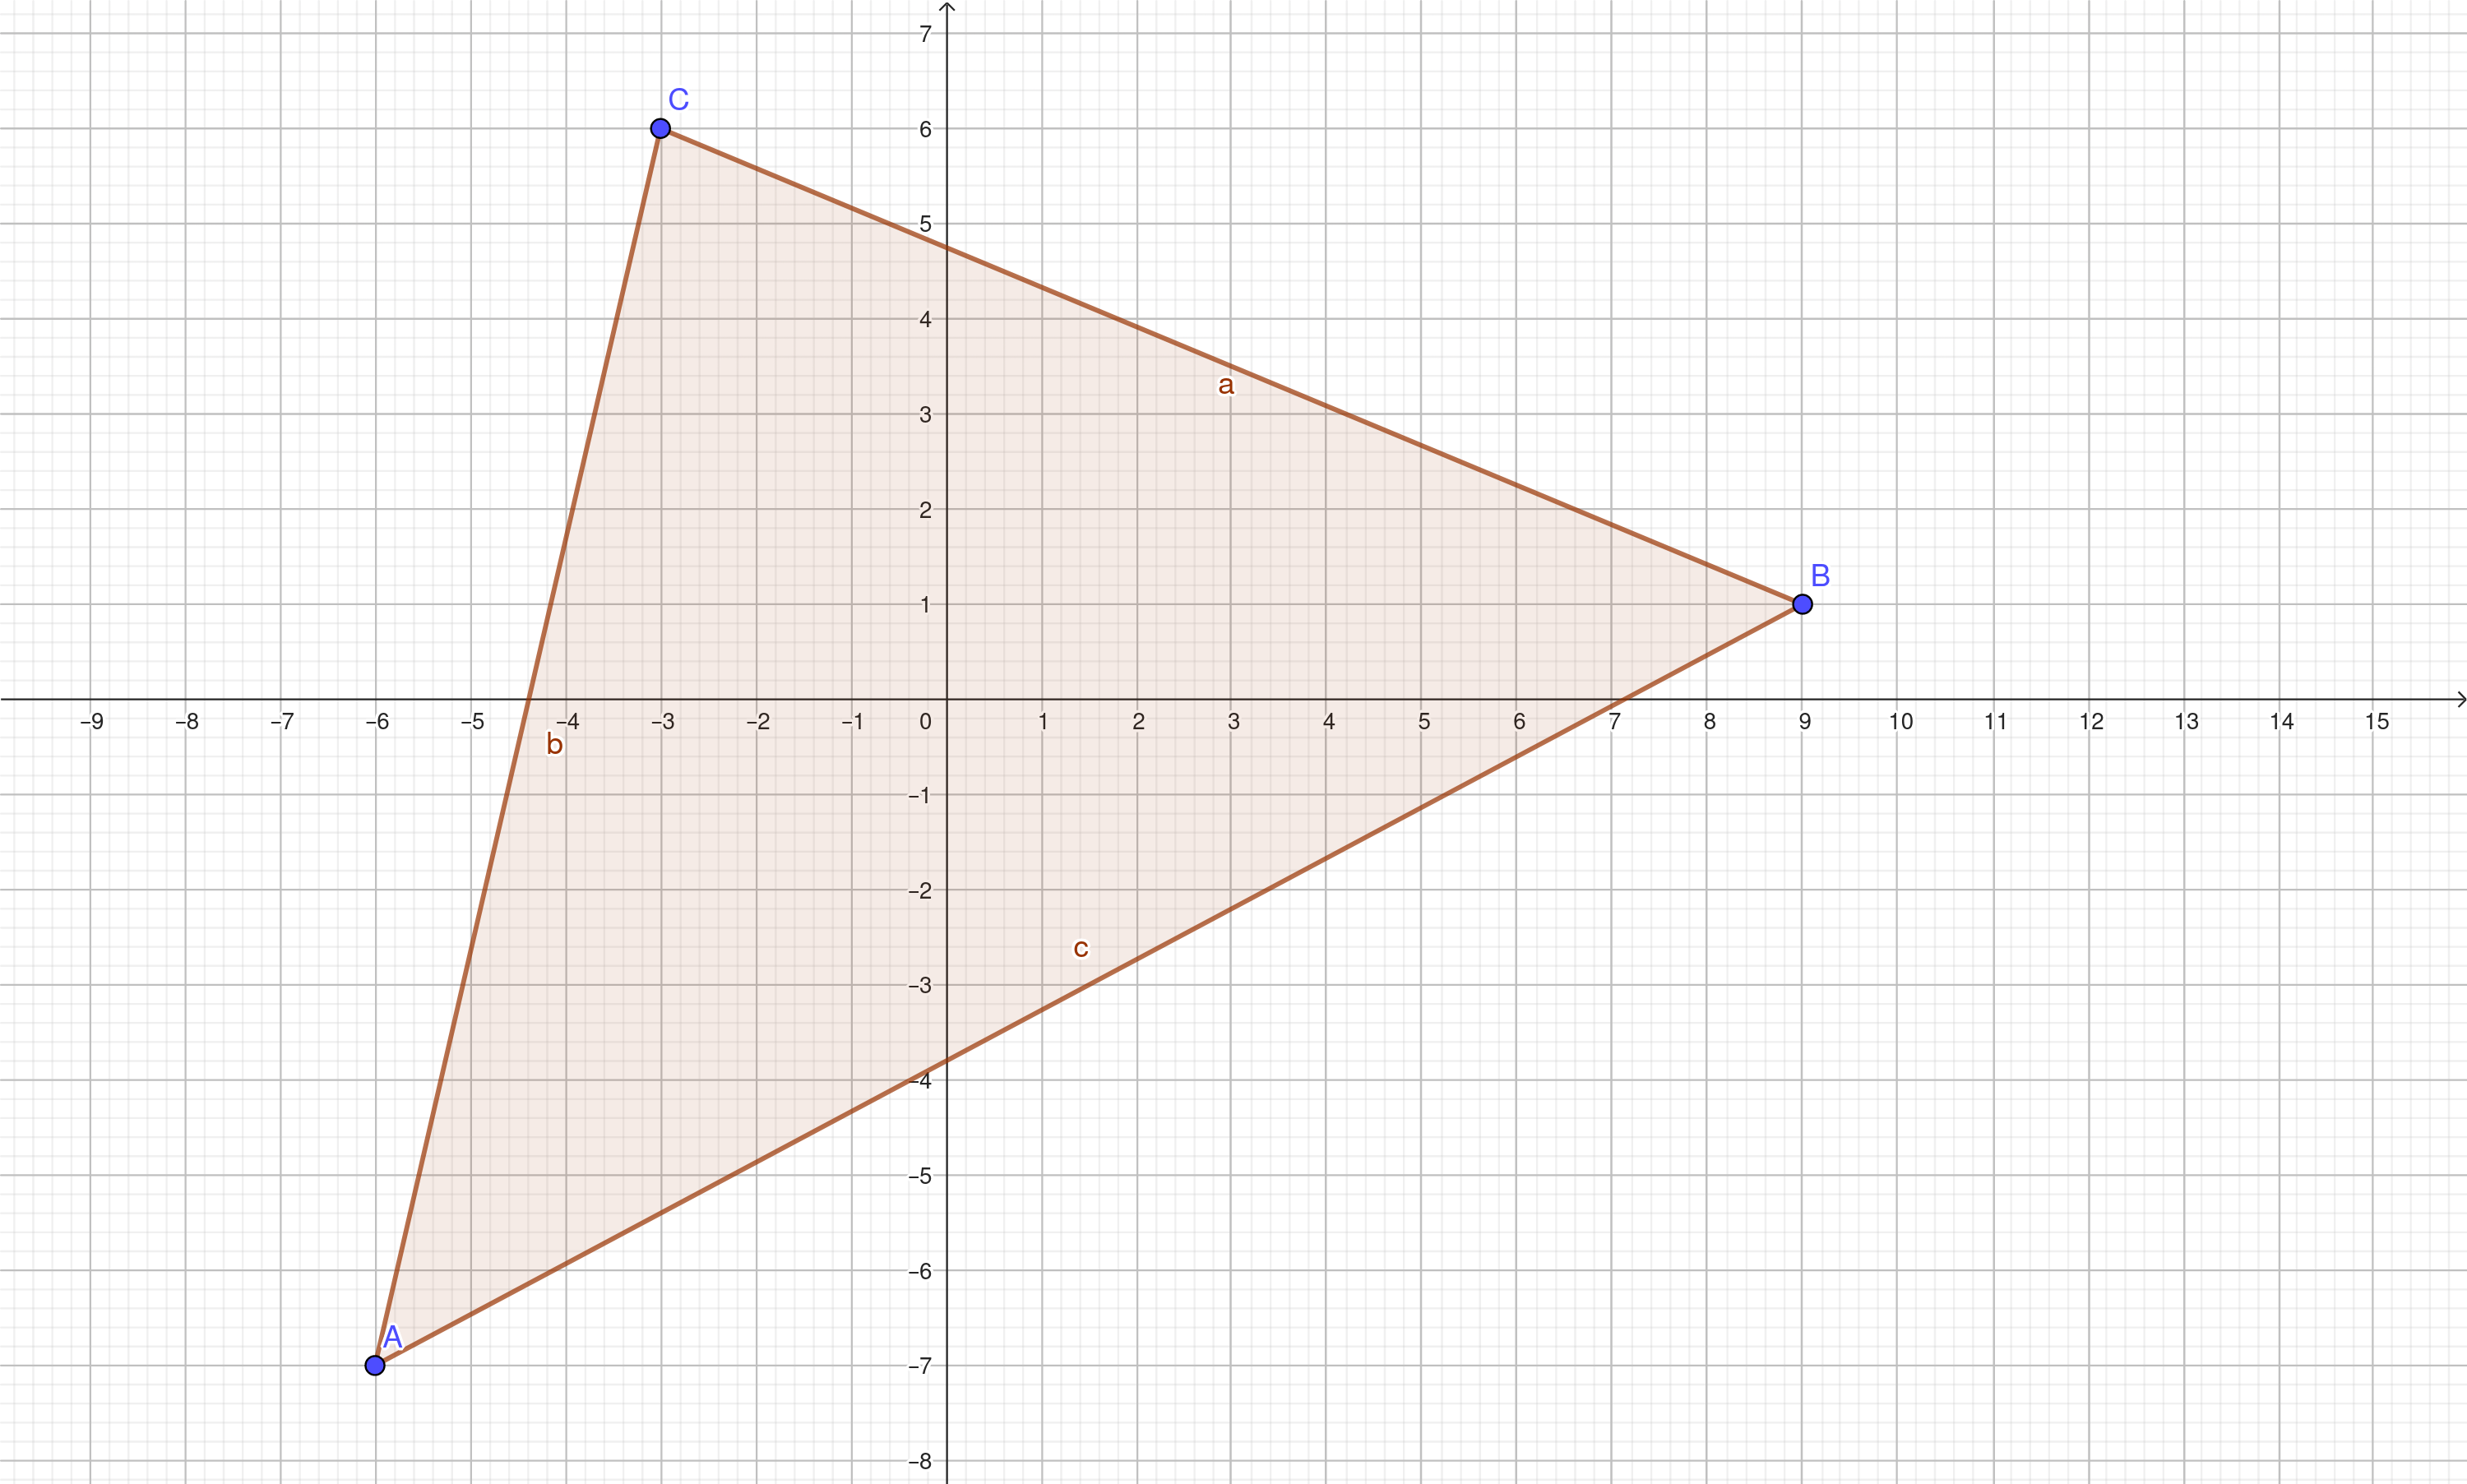
\includegraphics[width=\linewidth]{images/8-29-1.png}

\begin{align*}
    \vec{c} &= \vec{AB} \\ 
    &= \AB \\
    c &= |\vec{c}|  \\
    &= 17cm \\[20pt]
    \vec{a} &= \vec{BC} \\
    &= \BC \\
    a &= |\vec{a}| \\
    &= 13cm \\[20pt]
\end{align*}

\begin{align*}
    \cos({\beta}) &= \frac{\vec{a} \cdot \vec{c}}{|\vec{a}| * |\vec{b}|} \\
    &= \frac{\AB * \BC}{13 * 17}  \\
    &= -\frac{140}{221} \\
    &= \cosval \\[20pt]
    \beta &= \arccos(\cosval) \\
    &\approx \cosang^\circ \\[20pt]
    A &= \frac{a * c * \sin({\beta})}{2} \\
    &= \frac{13 * 17 * \sin({\cosang^\circ})}{2} \\
    &\approx 85.5cm^2
\end{align*}

\pagebreak

\paragraph{Answer:}
The obtuse value of $\beta$ ($\cosang^\circ$) was used instead of the acute value of $\beta$ 
($\cosanginv^\circ$). This didn't affect the result because 
$\sin(\beta)$ returns the same value for the obtuse and the acute value of $\beta$


\begin{align*}
    \sin(\alpha) &= \sin(180^\circ - \alpha) \\[20pt]
    \sin(\cosang^\circ) &= \sinofang \\
    \sin(\cosanginv^\circ) &= \sinofanginv 
\end{align*}

\pagebreak

\section*{8.31}
\paragraph{Specification:}
An isosceles triangle ABC, which is named in the mathematically positive direction, has the 
base AB with $A(-2|-1)$, $B(4|7)$ and the height h = 10E. Calculate the missing point C, the angle
$\phi$ which is enclosed by $\vec{AB}$ and $\vec{AC}$, and the area $A_{rea}$ of the triangle.

\def\height{10}

\def\A{\begin{pmatrix}
    -2 \\ 
    -1
\end{pmatrix}}

\def\B{\begin{pmatrix}
    4 \\ 
    7
\end{pmatrix}}

\def\AB{\begin{pmatrix}
    6 \\ 
    8
\end{pmatrix}}

\def\ABhalf{\begin{pmatrix}
    3 \\ 
    4
\end{pmatrix}}

\def\ABmid{\begin{pmatrix}
    1 \\ 
    3
\end{pmatrix}}

\def\ABnorm{\begin{pmatrix}
       -8 \\ 
        6
    \end{pmatrix}}

\def\ABnrommag{\sqrt{(-8)^2 + 6^2}}

\def\ABmidzero{\begin{pmatrix}
   -0.8 \\ 
    0.6
\end{pmatrix}}

\paragraph{Definitions:}
\begin{align*}
    h &= \height E \\
    A &= \A \\
    B &= \B \\
    \vec{c} &= \vec{AB} \\
    \vec{c_m} &= \vec{OA} + \frac{1}{2} \vec{c}
\end{align*}

\paragraph{Exercise:}
\begin{align*}
    \vec{c} &= \vec{B} - \vec{A} \\
    \vec{c} &= \B - \A \\
    \vec{c} &= \AB \\[20pt]
    \vec{c_m} &= \A + \frac{1}{2}\AB \\
    \vec{c_m} &= \A  + \ABhalf \\
    \vec{c_m} &= \ABmid \\[20pt]
    \vec{c_n} &= \ABnorm \\
    \vec{c_{n0}} &= \frac{1}{|\vec{c_n}|}\vec{c_n} \\
    \vec{c_{n0}} &= \frac{1}{\ABnrommag}\ABnorm \\
    \vec{c_{n0}} &= \frac{1}{10}\ABnorm \\
    \vec{c_{n0}} &= \ABmidzero \\[20pt]
    \vec{OC} &= \ABmid + \height\ABmidzero \\
    \vec{OC} &= \begin{pmatrix}
       -7 \\ 
        9
    \end{pmatrix}
\end{align*}

\end{document}
